\documentclass[12pt,a4paper]{article}
\usepackage[utf8]{inputenc}
\usepackage[bahasa]{babel}
\usepackage{geometry}
\usepackage{graphicx}
\usepackage{listings}
\usepackage{xcolor}
\usepackage[
    colorlinks=true,
    linkcolor=black,
    citecolor=black,
    urlcolor=blue
]{hyperref}


% Margin setting
\geometry{left=3cm, right=3cm, top=3cm, bottom=3cm}

% Code listing style
\definecolor{codegreen}{rgb}{0,0.6,0}
\definecolor{codegray}{rgb}{0.5,0.5,0.5}
\definecolor{codepurple}{rgb}{0.58,0,0.82}
\definecolor{backcolour}{rgb}{0.95,0.95,0.92}

\lstdefinestyle{pythonstyle}{
    backgroundcolor=\color{backcolour},   
    commentstyle=\color{codegreen},
    keywordstyle=\color{magenta},
    numberstyle=\tiny\color{codegray},
    stringstyle=\color{codepurple},
    basicstyle=\ttfamily\footnotesize,
    breakatwhitespace=false,         
    breaklines=true,                 
    captionpos=b,                    
    keepspaces=true,                 
    numbers=left,                    
    numbersep=5pt,                  
    showspaces=false,                
    showstringspaces=false,
    showtabs=false,                  
    tabsize=2,
    language=Python
}
\lstset{style=pythonstyle}

% Hyperlink setup
\hypersetup{
    colorlinks=true,
    linkcolor=black,
    urlcolor=blue,
}

\begin{document}

% ========== COVER PAGE ==========
\begin{titlepage}
    \centering
    \vspace*{2cm}
    

    {\LARGE\bfseries LAPORAN TUGAS BESAR\par}
    {\large Sistem/Teknologi Multimedia (IF25-40305)\par}
    \vspace{0.5cm}
    {\large Filter Kuis Matematika Interaktif dengan\par}
    {\large Hand Gesture Recognition (DO THE MATH!)\par}
    
    \vspace{1cm}
    
    % Logo ITERA
    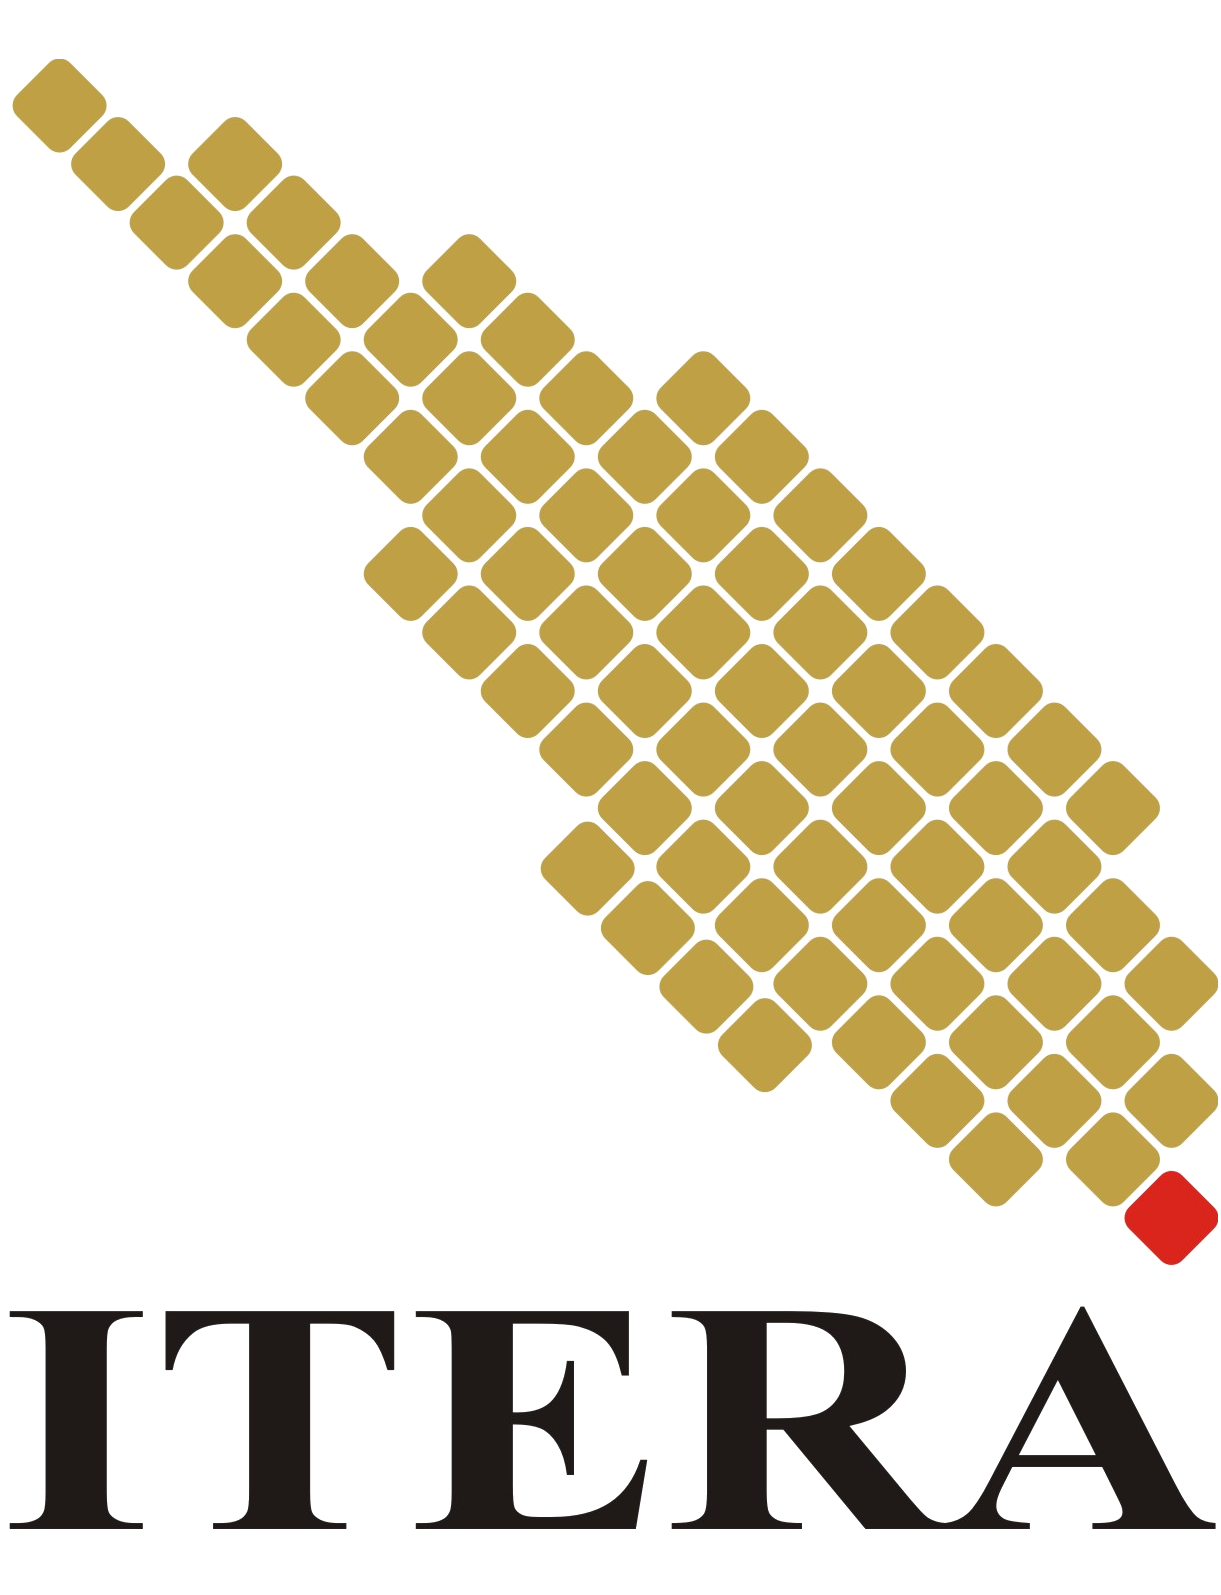
\includegraphics[width=6cm]{gambar/Logo_ITERA.png}\\[1cm]
    \vfill

    {\large
    \textbf{Disusun oleh:}\par
    \vspace{0.5cm}
    \begin{tabular}{ll}
        Tawakkal Rabbani Muhammad & (122140029)\\
        Naufal Harris Nurkhoirulloh & (122140040)\\
        Nashwa Putri Laisya & (122140180)\\
    \end{tabular}
    \par}
    
    \vfill
    
    \vspace{2cm}
    {\large
    \textbf{PROGRAM STUDI TEKNIK INFORMATIKA}\\
    \textbf{INSTITUT TEKNOLOGI SUMATERA}\\
    \textbf{2025}
    \par}
    
\end{titlepage}

% ========== TABLE OF CONTENTS ==========
\tableofcontents
\newpage

% ========== BAB 1 ==========
\section{Pendahuluan}
\subsection{Latar Belakang}
% Isi latar belakang di sini

\subsection{Rumusan Masalah}
% Isi rumusan masalah di sini

\subsection{Tujuan}
% Isi tujuan di sini

\subsection{Ruang Lingkup}
% Isi ruang lingkup di sini

\newpage


% ========== BAB 2 ==========
\section{Alat dan Bahan}
\subsection{Bahasa Pemrograman dan Lingkungan Pengembangan}
% Isi penjelasan bahasa pemrograman (Python) di sini


\subsection{Library dan Pustaka yang Digunakan}
% Isi library yang digunakan:
% - opencv-python
% - mediapipe
% - onnxruntime
% - numpy
% - cvzone
% - pygame


\subsection{Metode dan Algoritma}
% Isi penjelasan metode:
% - Estimasi Heart Rate (HR)
% - Estimasi Respiration Rate (RR)
% - Transformasi Fourier (FFT)

\newpage


% ========== BAB 3 ==========
\section{Penjelasan Sistem}

Bab ini menjabarkan struktur teknis dari perangkat lunak \textit{DO THE MATH!}. Pembahasan mencakup organisasi direktori proyek, prosedur instalasi dependensi, serta analisis mendalam mengenai logika pemrograman pada setiap modul utama, termasuk kelas dan fungsi yang membangun sistem interaksi \textit{gesture}, pengenalan angka, dan manajemen kuis.

\subsection{Struktur Folder Proyek}
Struktur folder dalam proyek ini menerapkan prinsip \textbf{modularitas}. Tujuannya adalah untuk memisahkan setiap tugas spesifik, seperti logika kuis, pengolahan gambar, kecerdasan buatan (AI), dan manajemen aset multimedia. Dengan struktur ini, proses pengembangan dan \textit{debugging} menjadi lebih mudah. Pembagian folder dan file utamanya adalah sebagai berikut:

\begin{enumerate}
    \item \textbf{main.py}: Berkas utama yang berfungsi sebagai inti dari aplikasi, menghubungkan ke kamera, logika permainan, dan antarmuka pengguna (\textit{User Interface}).
    \item \textbf{gesture\_tracking.py}: Modul untuk mendeteksi tangan dan mengenali \textit{gesture} jari (menggambar, \textit{submit}, hapus) menggunakan MediaPipe.
    \item \textbf{digit\_recognition.py}: Modul AI yang memproses gambar angka dari \textit{canvas} dan melakukan prediksi menggunakan model ONNX MNIST.
    \item \textbf{quiz\_manager.py}: Mengelola logika kuis, memuat soal dan jawaban, serta menghitung skor.
    \item \textbf{audio\_manager.py}: Mengelola pemutaran efek suara dan audio soal menggunakan Pygame.
    \item \textbf{confetti\_effect.py}: Sistem partikel untuk efek visual saat jawaban benar.
    \item \textbf{models/}: Menyimpan model \textit{Pre-trained} seperti \texttt{mnist-8.onnx}.
    \item \textbf{assets/}: Berisi aset audio (\texttt{.wav}) dan ikon (\texttt{.png}).
    \item \textbf{data/}: Berisi gambar soal dan audio soal.
\end{enumerate}

\subsection{Instalasi Library}
Agar program dapat berjalan dengan baik, pustaka yang tercantum dalam file \texttt{requirements.txt} harus diinstal terlebih dahulu. Pustaka utama yang digunakan meliputi \texttt{opencv-python}, \texttt{mediapipe}, \texttt{onnxruntime}, \texttt{pygame}, dan \texttt{numpy}. Instalasi dapat dilakukan dengan perintah berikut di terminal:

\begin{lstlisting}[language=bash, frame=single, basicstyle=\small\ttfamily]
pip install -r requirements.txt
\end{lstlisting}

\subsection{Modul main.py}
Modul ini adalah file utama yang menghubungkan dan menjalankan semua bagian sistem. Di dalamnya terdapat dua kelas utama yang menangani logika aplikasi dan tampilan visual.

\subsubsection{Kelas UIManager}
Kelas ini bertanggung jawab atas \textbf{menggambar semua tampilan kuis} di atas hasil tangkapan kamera.
\begin{itemize}
    \item \texttt{draw\_left\_panel}: Metode ini merender panel informasi di sisi kiri layar yang memuat instruksi permainan, skor terkini, serta indikator status \textit{charging} untuk mode menggambar.
    \item \texttt{draw\_question\_panel}: Bertugas menampilkan citra soal matematika pada posisi sudut kanan atas layar agar mudah dilihat pengguna tanpa menutupi area kerja utama.
    \item \texttt{show\_notification} \& \texttt{draw\_notification}: Sepasang metode untuk mengatur dan menampilkan pesan umpan balik sementara (seperti "BENAR!" atau "SALAH!") di bagian tengah bawah layar.
\end{itemize}

\subsubsection{Kelas MathQuizApp}
Merupakan kelas inti yang menginisialisasi sistem dan menjalankan \textit{loop} utama aplikasi.
\begin{itemize}
    \item \texttt{\_\_init\_\_}: Konstruktor yang menginisialisasi kamera, memuat model AI, serta menyiapkan instansi dari \textit{GestureController}, \textit{QuizManager}, dan \textit{AudioPlayer}.
    \item \texttt{process\_answer}: Metode logika yang dipanggil saat pengguna melakukan gestur \textit{submit}. Metode ini menghentikan input sementara, melakukan prediksi angka, memvalidasi jawaban dengan kunci jawaban, dan memicu efek audio visual yang sesuai.
    \item \texttt{run}: Metode utama yang menjalankan siklus pengambilan \textit{frame} kamera, pemrosesan deteksi tangan, pembaruan kanvas, serta pemanggilan fungsi \textit{rendering} UI secara \textit{real-time}.
\end{itemize}

\subsection{Modul gesture\_tracking.py}
Modul ini berfungsi untuk \textbf{membaca gerakan tangan kita} dan mengubahnya menjadi perintah digital, semuanya berkat bantuan library MediaPipe.

\subsubsection{Kelas GestureController}
Kelas ini mengelola logika pelacakan tangan dan penerjemahan posisi jari menjadi aksi pada kanvas.
\begin{itemize}
    \item \texttt{get\_hand\_info}: Metode pembungkus (\textit{wrapper}) untuk MediaPipe yang mendeteksi keberadaan tangan dan mengembalikan koordinat 21 titik \textit{landmark} serta status jari (terbuka/tertutup).
    \item \texttt{process\_gesture}: Inti dari logika interaksi. Metode ini menganalisis konfigurasi jari untuk menentukan mode:
    \begin{itemize}
        \item \textbf{1 Jari (Telunjuk)}: Mengaktifkan mode menggambar. Dilengkapi mekanisme \textit{charging} (penundaan) untuk mencegah coretan tidak sengaja.
        \item \textbf{4 Jari}: Memicu aksi \textit{submit} jawaban.
        \item \textbf{5 Jari}: Memicu aksi \textit{clear} untuk menghapus kanvas.
    \end{itemize}
    \item \texttt{is\_ready\_to\_draw}: Mengembalikan status boolean apakah waktu penundaan (\textit{charging time}) telah terpenuhi sehingga sistem mengizinkan penggambaran garis.
\end{itemize}

\subsection{Modul digit\_recognition.py}
Modul ini adalah bagian yang isinya fungsi-fungsi untuk \textbf{mengubah gambar tulisan tangan menjadi angka} yang bisa dibaca oleh program, menggunakan teknologi AI. Modul ini menggunakan pendekatan fungsional, bukan berbasis kelas.

\subsubsection{Fungsi-fungsi Utama}
\begin{itemize}
    \item \texttt{load\_model}: Mengunduh (jika belum ada) dan memuat model \texttt{mnist-8.onnx} menggunakan \texttt{onnxruntime.InferenceSession}.
    \item \texttt{find\_digit\_bboxes}: Melakukan segmentasi citra untuk menemukan lokasi angka pada kanvas. Metode ini menggunakan teknik kontur (\textit{contours}) OpenCV, menyaring \textit{noise} berdasarkan luas area, dan mengurutkan bounding box dari kiri ke kanan untuk mendukung pembacaan angka multi-digit (puluhan/ratusan).
    \item \texttt{preprocess\_single\_digit}: Melakukan pra-pemrosesan pada potongan citra angka. Langkah ini meliputi konversi ke \textit{grayscale}, \textit{thresholding}, penyesuaian rasio aspek, dan normalisasi ukuran menjadi $28 \times 28$ piksel agar sesuai dengan input yang diharapkan model MNIST.
    \item \texttt{recognize\_multi\_digit}: Fungsi orkestrator yang menggabungkan deteksi bounding box dan inferensi model untuk mengenali deretan angka sekaligus, menghasilkan string angka hasil prediksi (misalnya "12").
\end{itemize}

\subsection{Modul quiz\_manager.py}
Modul ini mengurus semua \textbf{logika kuis}, seperti menyimpan soal, jawaban, dan mengatur jalannya permainan. Tujuannya agar data soal terpisah dari bagian tampilan.

\subsubsection{Kelas QuizManager}
\begin{itemize}
    \item \texttt{\_\_init\_\_} \& \texttt{\_\_load\_questions}: Memindai folder \texttt{data/} untuk memuat pasangan file gambar (\texttt{.png}) dan audio (\texttt{.wav}) secara otomatis, serta membaca kunci jawaban dari \texttt{answers.txt}.
    \item \texttt{check\_answer}: Membandingkan jawaban hasil prediksi AI dengan kunci jawaban yang tersimpan. Metode ini juga memperbarui statistik skor pemain.
    \item \texttt{next\_question}: Menggeser pointer indeks ke soal berikutnya dalam antrean.
    \item \texttt{get\_score}: Mengembalikan statistik performa pemain berupa jumlah jawaban benar, total soal yang telah dijawab, dan persentase keberhasilan.
\end{itemize}

\subsection{Modul audio\_manager.py}
Modul ini menangani aspek suara aplikasi, dari narasi soal hingga efek suara, menggunakan pustaka \texttt{pygame.mixer}.

\subsubsection{Kelas AudioPlayer}
\begin{itemize}
    \item \texttt{play\_question\_audio}: Memutar rekaman narasi soal. Metode ini bersifat \textit{non-blocking}, sehingga program tetap berjalan lancar saat audio diputar.
    \item \texttt{play\_sound\_effect}: Memutar efek suara pendek seperti notifikasi salah atau benar.
    \item \texttt{play\_correct\_sequence}: Menjalankan urutan audio khusus untuk jawaban benar, yaitu memutar suara "correct" diikuti oleh suara tepuk tangan ("applause") secara berurutan.
\end{itemize}

\subsection{Modul confetti\_effect.py}
Modul ini mengimplementasikan sistem partikel sederhana untuk memberikan efek visual yang meriah saat pengguna berhasil menjawab dengan benar.

\subsubsection{Kelas Confetti}
Merepresentasikan satu partikel tunggal. Kelas ini memiliki properti posisi, kecepatan, warna, rotasi, dan bentuk. Metode \texttt{update} di dalamnya menerapkan simulasi fisika sederhana (gravitasi dan resistansi udara) untuk menciptakan efek jatuh yang natural.

\subsubsection{Kelas ConfettiSystem}
Bertindak sebagai pengelola (\textit{manager}) ribuan objek partikel.
\begin{itemize}
    \item \texttt{generate\_burst}: Menciptakan ledakan partikel baru dalam jumlah banyak pada posisi acak di bagian atas layar.
    \item \texttt{update} \& \texttt{draw}: Memperbarui posisi seluruh partikel aktif dan menggambarnya ke layar pada setiap \textit{frame}.
\end{itemize}

\newpage

% ========== BAB 4 ==========
\section{Hasil}
\subsection{Hasil Implementasi}

\subsection{Analisis Hasil}
% Isi analisis hasil
% - Performa aplikasi
% - Akurasi deteksi
% - dll

\newpage


% ========== BAB 5 ==========
\section{Kesimpulan dan Saran}

\subsection{Kesimpulan}
Berdasarkan proses perancangan, implementasi, hingga pengujian yang telah dilakukan pada aplikasi \textit{DO THE MATH!}, dapat ditarik beberapa kesimpulan sebagai berikut:

\begin{enumerate}
    \item \textbf{Integrasi Sistem Berhasil Dilakukan:}
    Aplikasi berhasil menggabungkan teknologi \textit{Computer Vision} (MediaPipe) dan kecerdasan buatan (ONNX Runtime) menjadi satu kesatuan sistem yang utuh. Sistem mampu berjalan secara \textit{real-time} melalui \textit{webcam} untuk mendeteksi gerakan tangan sekaligus mengenali tulisan angka di udara tanpa kendala integrasi yang berarti.

    \item \textbf{Efektivitas Interaksi Gesture:}
    Implementasi logika \textit{gesture control} dengan mekanisme \textit{charging time} (waktu tunggu) terbukti efektif dalam meningkatkan pengalaman pengguna. Fitur ini berhasil meminimalisir terjadinya coretan garis yang tidak disengaja saat pengguna baru mengangkat tangan, sehingga proses menggambar menjadi lebih terkontrol dan natural.

    \item \textbf{Kemampuan Pengenalan Angka:}
    Modul \textit{Digit Recognition} yang dilengkapi dengan tahapan \textit{preprocessing} citra (seperti \textit{thresholding} dan operasi morfologi) mampu mengenali input angka tulisan tangan dengan cukup baik. Algoritma pengurutan kontur (\textit{contour sorting}) juga berhasil diterapkan untuk menangani jawaban yang terdiri dari dua digit (multi-digit), sehingga sistem tidak terbatas pada jawaban satuan saja.

    \item \textbf{Ketergantungan pada Lingkungan:}
    Meskipun sistem berfungsi dengan baik secara logika, performanya di dunia nyata masih sangat dipengaruhi oleh faktor eksternal, terutama pencahayaan. Kondisi minim cahaya dapat menyebabkan \textit{jitter} (getaran) pada deteksi jari, yang berdampak pada kerapian garis tulisan di kanvas virtual.
\end{enumerate}

\subsection{Saran}
Pengembangan aplikasi ini masih memiliki ruang untuk perbaikan dan penyempurnaan di masa mendatang. Berikut adalah beberapa saran yang dapat dipertimbangkan untuk pengembangan selanjutnya:

\begin{enumerate}
    \item \textbf{Peningkatan Akurasi Model:}
    Disarankan untuk melatih ulang model atau menggunakan dataset yang lebih variatif (termasuk variasi tulisan tangan yang miring atau tidak standar) guna mengurangi kesalahan prediksi pada angka yang memiliki bentuk mirip, seperti angka 4 dan 9.

    \item \textbf{Penanganan Kondisi Pencahayaan:}
    Untuk mengatasi masalah \textit{jitter} pada kondisi kurang cahaya, dapat ditambahkan algoritma \textit{stabilizer} atau filter tambahan (seperti Kalman Filter) pada koordinat jari agar garis yang dihasilkan tetap halus meskipun input kamera sedikit bergetar.

    \item \textbf{Variasi Soal Matematika:}
    Saat ini sistem berfokus pada operasi penjumlahan sederhana. Kedepannya, bank soal dapat diperluas untuk mencakup operasi pengurangan, perkalian, dan pembagian, serta penyesuaian tingkat kesulitan dinamis berdasarkan skor pengguna.

    \item \textbf{Optimasi untuk Spesifikasi Rendah:}
    Meskipun sudah cukup ringan, optimasi kode lebih lanjut dapat dilakukan agar aplikasi dapat berjalan lebih lancar pada perangkat dengan spesifikasi perangkat keras yang sangat terbatas.
\end{enumerate}

\newpage


% ========== LAMPIRAN ==========
\section{Lampiran}

\subsection{Lampiran A: Dokumentasi Github}

\subsubsection{Link Repository}
% Isi link Github repository di sini
% Contoh: https://github.com/username/DO-THE-MATH


\subsubsection{Dokumentasi Commit dan Kontribusi}
% Isi dokumentasi commit dari setiap anggota
% Screenshot commit history jika perlu


\subsection{Lampiran B: Penggunaan AI dalam Proyek}

\subsubsection{AI Tools yang Digunakan}
% Isi AI tools yang digunakan (Gemini, ChatGPT, dll)
% Contoh:
% - Google Gemini untuk ...
% - ChatGPT untuk ...


\subsubsection{Link Dokumentasi Penggunaan AI}
% Isi link ke chat history AI
% Contoh:
% - Gemini 1: https://...
% - ChatGPT: https://...


\subsubsection{Screenshot Penggunaan AI}
% Tambahkan screenshot chat dengan AI
% \begin{figure}[h]
% \centering
% \includegraphics[width=0.8\textwidth]{gambar/ai_screenshot.png}
% \caption{Screenshot penggunaan AI}
% \end{figure}


\subsection{Lampiran C: Kode Program Lengkap}

\subsubsection{File main.py}
% Isi kode lengkap main.py
% \begin{lstlisting}[caption=main.py]
% # Paste kode di sini
% \end{lstlisting}


\subsubsection{File digit\_recognition.py}
% Isi kode lengkap digit_recognition.py


\subsubsection{File gesture\_tracking.py}
% Isi kode lengkap gesture_tracking.py


% Tambahkan file-file lain sesuai kebutuhan


\subsection{Lampiran D: Screenshot Tambahan}

\subsubsection{Screenshot Proses Development}
% Screenshot selama proses development


\subsubsection{Screenshot Testing}
% Screenshot saat testing aplikasi


\subsubsection{Screenshot Error dan Debugging}
% Screenshot error dan cara debugging (opsional)

\newpage


% ========== REFERENCES ========== 
\bibliographystyle{IEEEtran}
\bibliography{references}

\end{document}